\chapter{Introduction}\label{intro}
(incomplete)
In this chapter we briefly discuss about motifs,
what are they and why are we interested in them. 


\section{What are Motifs}
Motif\index{Motif} usually means a pattern. For any sequence
of objects to be called a pattern, it has to have at least
more than one instance. To define more precisely, a motif
should have significantly higher occurrence in a given array
or list compared to what you would obtain in a randomized
array of same components. Here array means an arranged set
such as a genome or a protein structure. Genome is an array
of nucleotides and protein structure is an array of amino acids.



\subsection{Sequence Motifs}
By sequence motif\index{Motif!Sequence Motif} we mean a pattern
of nucleotide or amino acid that has specific biological
significance. In other words, they are pattern of a DNA array or
protein sequence. They may be also called regulatory sequence
motifs. This kind of motifs are commonly studied in bioinformatics.
They are becoming increasingly important in the analysis of gene
regulation. In our thesis we will only discuss about this type of motifs.


\subsection{Structural Motifs}
Structural motifs\index{Motif!Structural Motif} are a super-secondary
structure in a chain like biological molecules such as protein.
It is formed by three dimensional alignment of amino acids
which may not be adjacent. 


\section{Regulatory Motifs in DNA}
Regulatory motifs\index{Regulatory Motifs} are some short nucleotide
sequence that regulates the expression of genes such as controlling
the situations under which the genes will be turned on or off.
For example:~\cite{jones2004introduction} Fruit flies have a small
set of \textit{immunity genes} that are dormant
in their genome. But when its organisms get infected somehow the genes
got switched on. It turns out that many immunity genes in
the fruit fly genome have strings that are reminiscent of TCGGGGATTTCC,
located upstream of the genes start. This string are called $ _{NF-\kappa}$B
binding sites which are important examples of regulatory motifs. Proteins
known as \textit{transcription factors} bind to these motifs, encouraging
RNA polymerase to transcribe the downstream genes.


\subsection{Regulatory Regions}
As discussed in~\cite{Riethoven2010} regulation of gene expression
is an essential part of every organism. Certain regions,
called cis-regulatory elements, on the DNA are footprints for
the trans-acting proteins involved in transcription. DNA
regions involved in transcription and transcriptional regulation
are called regulatory regions (RR).\index{Regulatory Motifs!Regulatory Regions}
Every gene contains a RR typically
stretching 100-1000 bp upstream of the transcriptional start site.
In  \Cref{fig:rr} we see the structure of a eukaryotic protein
coding gene. Regulatory sequence controls when and where expression
occurs for the protein coding region (red). Promoter and enhancer
regions (yellow) regulate the transcription of the gene into a
pre-mRNA which is modified to remove introns (light grey) and
add a 5' cap and ploy-A tail (dark grey). The mRNA 5' and 3'
untranslated regions (blue) regulate translation into the
final protein product.


\begin{figure}[!tb]
	\centering
	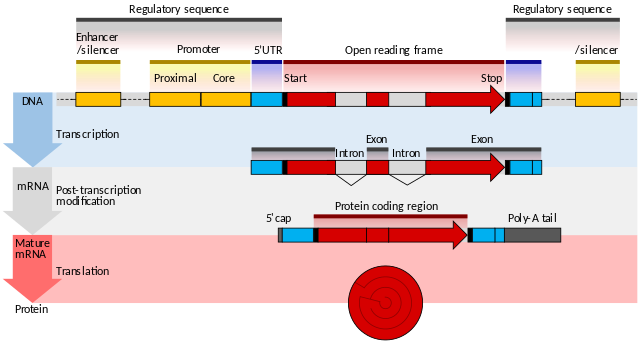
\includegraphics[width=0.9\textwidth]{figures/rr}
	\caption{The structure of a eukaryotic protein-coding gene.}
	\label{fig:rr}
\end{figure}


\subsection{Transcription Factor Binding Sites}
\index{Regulatory Motifs!Transcription Factor Binding Sites}
A transcription factor (TF) is a protein that can bind to DNA
and regulate gene expression. The region of the gene to which
TF binds is called a transcription factor binding site (TFBS).
TFs influence gene expression by binding to a specific location
in the respective gene’s regulatory region which is known as
TFBSs or motifs.~\cite{wei2007comparative} TFBS can be located
anywhere within the RR. TFBS may vary slightly across different
regulatory regions since non-essential bases could mutate.
TFBSs are a part of either the promoter or enhancer region of a gene.
A promoter sits upstream and contains three important regions-
the regulatory protein binding site, the transcription factor
binding site, and the RNA polymerase binding site.
In \Cref{fig:tfbs} we see a picture of promoter
and enhancer. An enhancer is usually far upstream of a gene.

\begin{figure}[!tb]
	\centering
	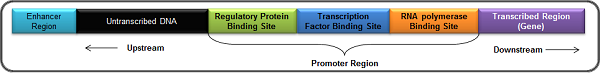
\includegraphics[width=0.9\textwidth]{figures/tfbs}
	\caption{Transcription Factor Binding Sites.}
	\label{fig:tfbs}
\end{figure}


\section{Motifs Logos}
Motifs can mutate at the non important bases. Motif logo\index{Motifs!Motifs Logos}
is one type of representation of the variable and fixed regions of
the motif. 


\section{Problem Description}
\section{Review of Literature}
\section{Why Study Motifs}


\endinput

%See these examples:
%\begin{itemize}
%	\item 
%	\item \Cref{fig:sample} is a sample figure.
%	\item \Cref{tab_our} is a table.
%	\item \Cref{sec:cite} in \Cref{ch:citations} shows some examples of
%	  citations.
%\end{itemize}

%\section{How to Write a Section}
%
%This is for writing section.
%
%\section{How to Add Table and Figures}\label{contribution}
%You should refer a figure as, ``\Cref{fig:sample} is a sample
%figure''.
%
%\begin{figure}[!tb]
%  \centering
%  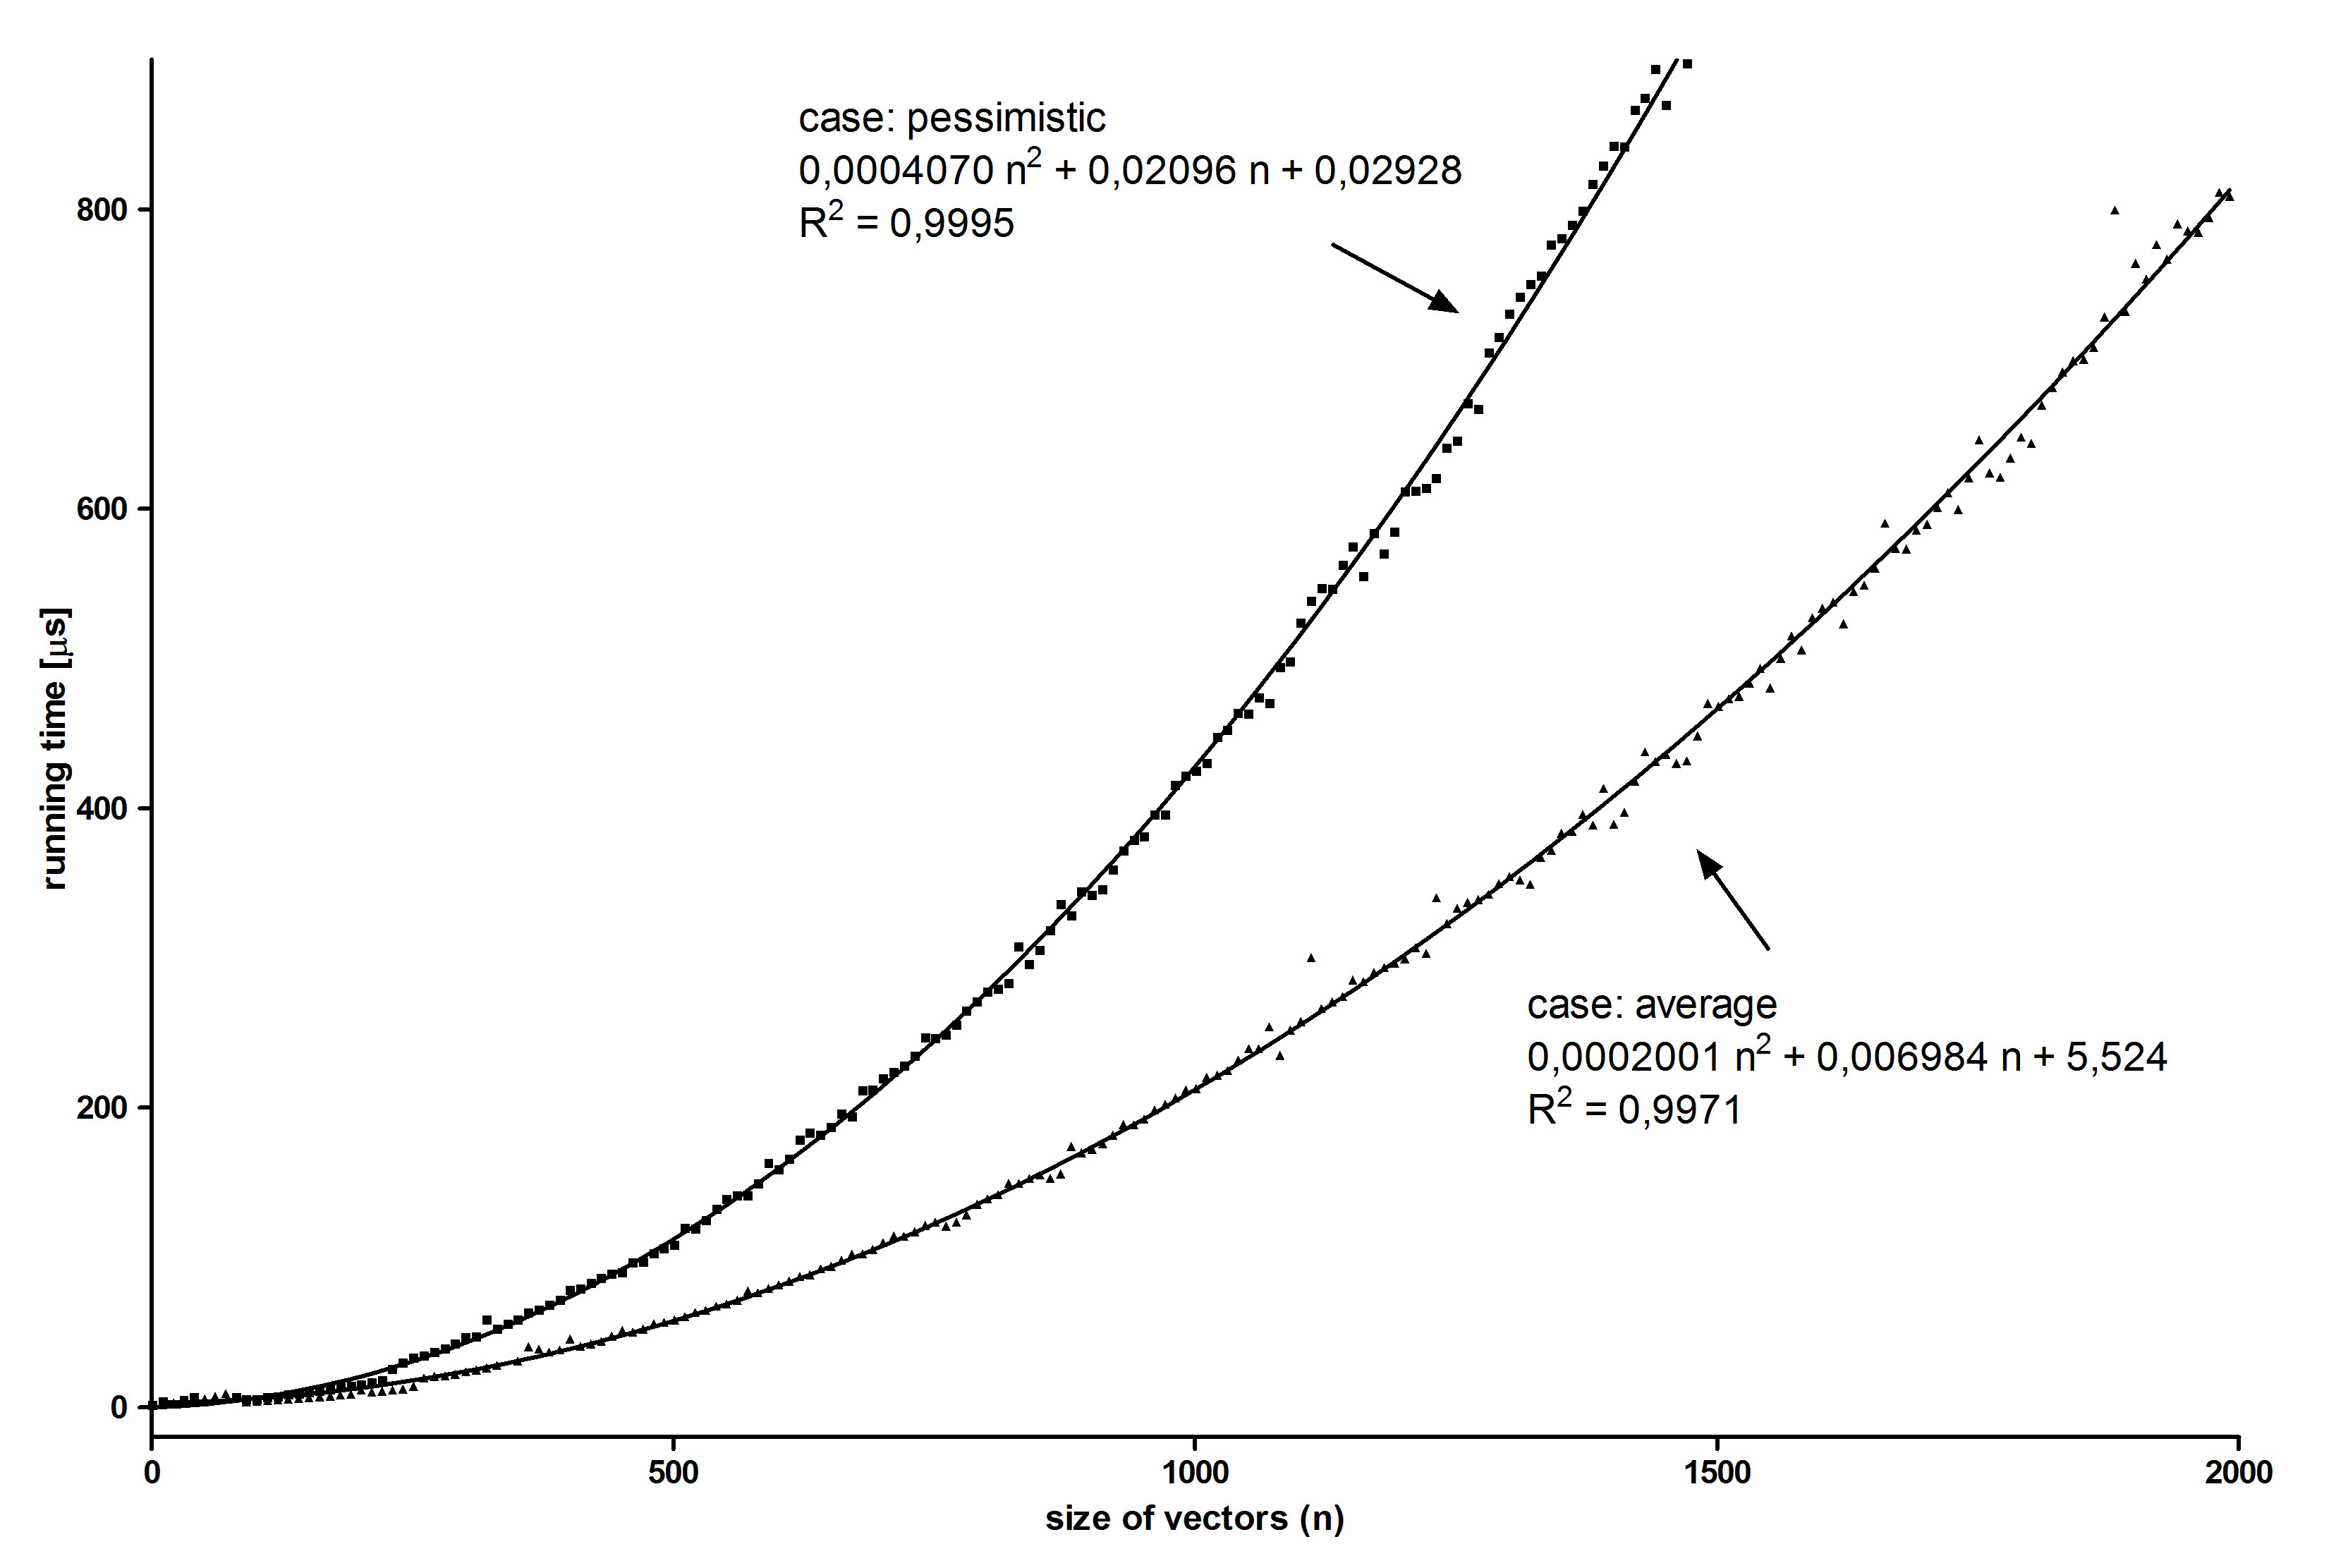
\includegraphics[width=0.9\textwidth]{figures/sample}
%  \caption{This is a sample figure.}
%  \label{fig:sample}
%\end{figure}
%
%				
%Then we applied same test cases to our modified algorithm i.e.\ the
%heuristic algorithm with our new operation \textit{Block Reversal}. The
%performance is shown in \Cref{tab_our}.


%\begin{table}[!tb]
%	\begin{center}
%		\caption{Degenerate nucleotide code}
%		\label{tab_nucleotide_code}
%		
%		\begin{tabular}{|l|r|r|r|}
%			
%			\hline
%			IUB	& Nucleotides	& Name	& [pA,pc,pG,pT]\\	
%			\hline
%			
%			A 	& A & Adenine & $ [1, 0, 0, 0] $ \\
%			C	&C	&Cytosine	&$ [0, 1, 0, 0] $\\
%			
%			G	&G	&Glutamine	 &$[0, 0, 1, 0] $\\
%			
%			T	&T	&Tyrosine	&$ [0, 0, 0, 1] $\\
%			
%			S	&C or G		&Strong		&$ [0, \frac{1}{2}, \frac{1}{2}, 0] $\\
%			
%			W	&A or T		&Weak	&$ [\frac{1}{2}, 0, 0, \frac{1}{2}] $\\
%			
%			R	&A or G	&PuRine		&$ [\frac{1}{2}, 0, \frac{1}{2}, 0] $\\
%			
%			Y	&C or T	&pYrimidine		&$ [0, \frac{1}{2}, 0, \frac{1}{2}] $\\
%			
%			M	&A or C	&aMino group	&$ [\frac{1}{2}, \frac{1}{2}, 0, 0] $\\
%			
%			K	&G or T		&Keto group		&$ [0, 0, \frac{1}{2}, \frac{1}{2}] $\\
%			
%			B	&C or G or T		&Not A	&$ [0, \frac{1}{3}, \frac{1}{3}, \frac{1}{3}] $\\
%			
%			D	&A or G or T	&Not C	&$ [\frac{1}{3}, 0, \frac{1}{3},\frac{1}{3}] $\\
%			
%			H	&A or C or T  &Not G  &$ [\frac{1}{3}, \frac{1}{3}, 0, \frac{1}{3}] $\\
%			
%			V	&A or C or G 	&Not T &$ [\frac{1}{3}, \frac{1}{3}, \frac{1}{3}, 0] $\\
%			
%			N	&A, C, G or T 	&aNy base &$ [\frac{1}{4}, \frac{1}{4},\frac{1}{4},\frac{1}{4}] $\\
%			\hline
%		\end{tabular}
%	\end{center}
%	
%\end{table}


%\begin{table}[!tb]
%  \begin{center}
%    \caption{Performance table of \emph{Block reversal} in a heuristic algorithm ($n=20$)}
%    \label{tab_our}
%
%    \begin{tabular}{|l|r|r|r|r|r|r|r|r|r|r|r|r|r|}
%      \hline
%      $\alpha$     & $\alpha n$ & \multicolumn{11}{c|}{Test Cases} & \multicolumn{1}{c|}{Average \# of}                                     \\
%      \cline{3-13} &            & 1                                & 2  & 3  & 4  & 5  & 6  & 7  & 8  & 9  & 10 & 11 & calculated operation \\
%      \hline
%      0.1        & 2          & 2                                & 2	& 2  & 2  & 2  & 2  & 2  & 2  &	2  & 2	& 2  & 2                    \\
%      0.2        & 4          & 4                                & 4	& 5  & 2  & 4  & 4  & 4  & 4  &	2  & 4	& 4  & 3.73                 \\
%      0.3        & 6          & 5                                & 6	& 6  & 6  & 6  & 7  & 6  & 5  &	6  & 6	& 6  & 5.91                 \\
%      0.4        & 8          & 7                                & 8	& 5  & 6  & 7  & 6  & 6  & 7  &	8  & 8	& 7  & 6.82                 \\
%      0.5        & 10         & 9                                & 10	& 6  & 12 & 10 & 8  & 10 & 10 &	7  & 7	& 10 & 9                    \\
%      0.6        & 12         & 9                                & 12	& 16 & 10 & 12 & 12 & 9  & 11 &	12 & 9	& 12 & 11.27                \\
%      0.7        & 14         & 13                               & 7	& 18 & 15 & 14 & 8  & 13 & 11 &	13 & 13	& 14 & 12.64                \\
%      0.8        & 16         & 10                               & 17	& 14 & 16 & 13 & 16 & 13 & 11 &	13 & 17	& 13 & 13.91                \\
%      0.9        & 18         & 14                               & 16	& 15 & 12 & 15 & 11 & 15 & 11 &	15 & 12	& 12 & 13.45                \\
%      1          & 20         & 18                               & 11	& 13 & 11 & 13 & 15 & 17 & 17 &	13 & 18	& 12 & 14.36                \\
%      \hline
%    \end{tabular}
%  \end{center}
%\end{table}
%

